%!TEX root = htm.tex
\section{Progressive HyTM must perform incremental validation}
\label{sec:lb}
%
%
\begin{figure*}[!ht]
\begin{center}
	\subfloat[Slow-path transaction $T_{\phi}$ performs $i-1$ distinct t-reads followed by the t-read of $X_i$ that returns value $nv$ 
	writtten by fast-path transaction $T_i$\label{sfig:inv-1}]{\scalebox{0.6}[0.6]{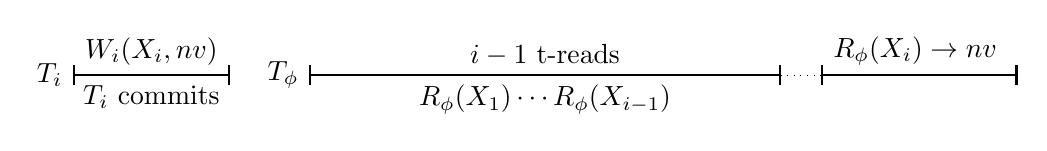
\begin{tikzpicture}
\node (r1) at (3,0) [] {};
\node (r2) at (7.7,0) [] {};

\node (w1) at (-2,0) [] {};


\draw (r1) node [below] {\normalsize {$R_{\phi}(X_1) \cdots R_{\phi}(X_{i-1})$}};
\draw (r1) node [above] {\normalsize {$i-1$ t-reads}};

\draw (r2) node [above] {\normalsize {$R_{\phi}(X_i)\rightarrow nv$}};

\draw (w1) node [above] {\normalsize {$W_i(X_i,nv)$}}; 
\draw (w1) node [below] {\normalsize {$T_i$ commits}};


\begin{scope}   
\draw [|-|,thick] (0,0) node[left] {$T_{\phi}$} to (6,0);
\draw [|-|,thick] (6.5,0) node[left] {} to (9,0);
\draw [-,dotted] (0,0) node[left] {} to (9,0);
\end{scope}
%
%
\begin{scope}   
%\draw [|-|,thick] (0,0) node[left] {$T_k$} to (6,0);
\draw [|-|,thick] (-3,0) node[left] {$T_i$} to (-1,0);
\end{scope}
%
\end{tikzpicture}
}}
        \\
        \vspace{1mm}
	\subfloat[Fast-path transaction $T_i$ does not contend with any of the $i-1$ t-reads performed by $T_{\phi}$;
	this execution is indistinguishable to $T_{\phi}$ from \ref{sfig:inv-1} and t-read of $X_i$ must return $nv$\label{sfig:inv-2}]{\scalebox{0.6}[0.6]{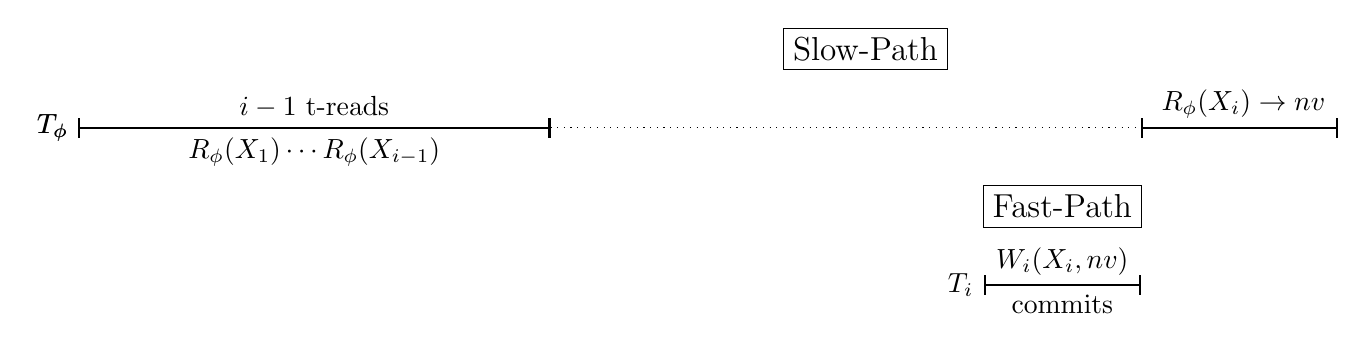
\begin{tikzpicture}
\node (r1) at (3,0) [] {};
%\node (r2) at (7.7,0) [] {};
\node (r3) at (14.8,0) [] {};

%\node (w1) at (7.5,-2) [] {};

\node (w2) at (12.5,-2) [] {};

\draw (r1) node [below] {\normalsize {$R_{\phi}(X_1) \cdots R_{\phi}(X_{i-1})$}};
\draw (r1) node [above] {\normalsize {$i-1$ t-reads}};

\draw (w2) node [above] {\normalsize {$W_{i}(X_{i},nv)$}}; 
\draw (w2) node [below] {\normalsize {commits}};

\draw (r3) node [above] {\normalsize {$R_{\phi}(X_{i})\rightarrow nv$}};
\node[draw,align=left] at (10,1) {{\large Slow-Path}};
\node[draw,align=left] at (12.5,-1) {{\large Fast-Path}};


\begin{scope}   
\draw [|-|,thick] (0,0) node[left] {$T_{\phi}$} to (6,0);
\draw [|-|,dotted] (0,0) node[left] {$T_{\phi}$} to (16,0);
\draw [|-|,thick] (13.5,0) node[left] {} to (16,0);
\end{scope}
%
%
\begin{scope}   
%\draw [|-|,thick] (0,0) node[left] {$T_k$} to (6,0);
\draw [|-|,thick] (11.5,-2) node[left] {$T_i$} to (13.5,-2);
\end{scope}
%
\end{tikzpicture}
%}}
	\\
	\vspace{1mm}
	\subfloat[To distinguish the $i-1$ different executions, t-read of $X_i$ by $T_{\phi}$ is forced
	to access $i-1$ different base objects\label{sfig:inv-3}]{\scalebox{0.6}[0.6]{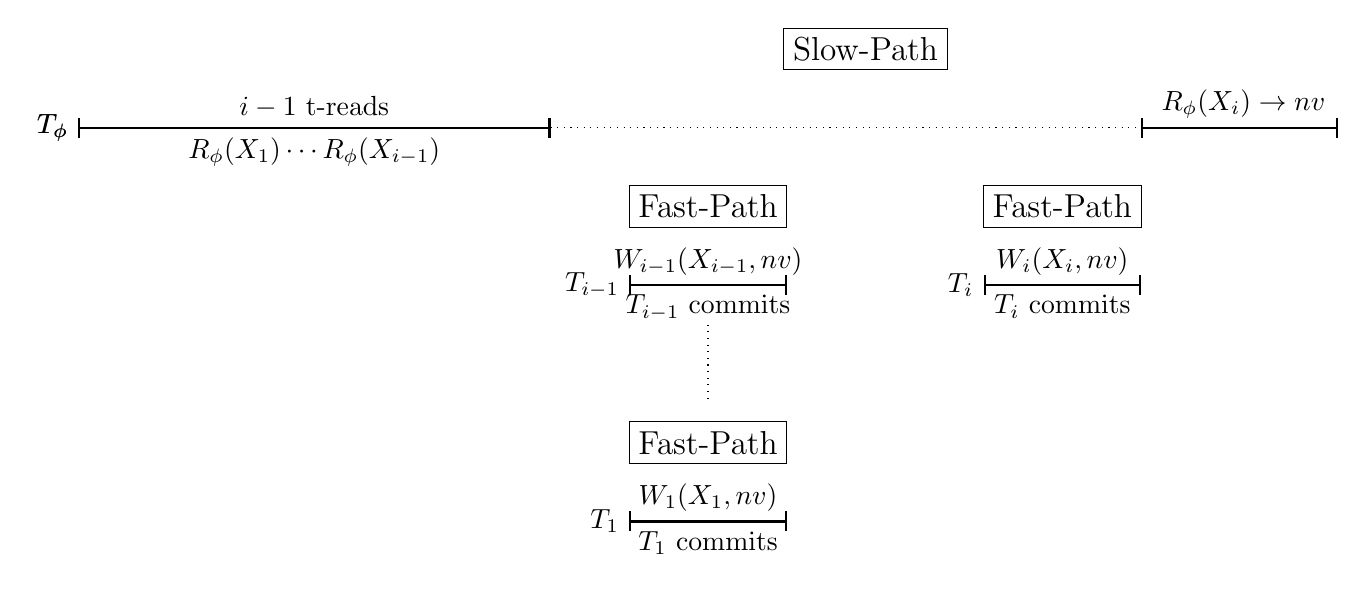
\begin{tikzpicture}
\node (r1) at (3,0) [] {};
%\node (r2) at (7.7,0) [] {};
\node (r3) at (14.8,0) [] {};


\node (w2) at (12.5,-2) [] {};
\node (w3) at (8,-2) [] {};
\node (w4) at (8,-5) [] {};


\draw (r1) node [below] {\normalsize {$R_{\phi}(X_1) \cdots R_{\phi}(X_{i-1})$}};
\draw (r1) node [above] {\normalsize {$i-1$ t-reads}};

\draw (w2) node [above] {\normalsize {$W_{i}(X_{i},nv)$}}; 
\draw (w2) node [below] {\normalsize {$T_{i}$ commits}};

\draw (w3) node [above] {\normalsize {$W_{i-1}(X_{i-1},nv)$}}; 
\draw (w3) node [below] {\normalsize {$T_{i-1}$ commits}};

\draw (w4) node [above] {\normalsize {$W_{1}(X_{1},nv)$}}; 
\draw (w4) node [below] {\normalsize {$T_{1}$ commits}};

\draw (r3) node [above] {\normalsize {$R_{\phi}(X_{i})\rightarrow nv$}};
\node[draw,align=left] at (10,1) {{\large Slow-Path}};
\node[draw,align=left] at (12.5,-1) {{\large Fast-Path}};
\node[draw,align=left] at (8,-1) {{\large Fast-Path}};
\node[draw,align=left] at (8,-4) {{\large Fast-Path}};
\begin{scope}   
\draw [|-|,thick] (0,0) node[left] {$T_{\phi}$} to (6,0);
\draw [|-|,dotted] (0,0) node[left] {$T_{\phi}$} to (16,0);
\draw [|-|,thick] (13.5,0) node[left] {} to (16,0);
\end{scope}
%
%
\begin{scope}   
\draw [|-|,thick] (7,-2) node[left] {$T_{i-1}$} to (9,-2);
\draw [|-|,thick] (11.5,-2) node[left] {$T_i$} to (13.5,-2);
\draw [-,dotted] (8,-2.5)  to (8,-3.5);
\draw [|-|,thick] (7,-5) node[left] {$T_1$} to (9,-5);

\end{scope}
%
\end{tikzpicture}
%}}
	\caption{Proof steps for Theorem~\ref{th:impossibility}
        \label{fig:indis}} 
\end{center}
\end{figure*}
%
In this section, we show that it is impossible to implement opaque \emph{progressive} HyTMs with \emph{invisible reads}
with $O$(1) step-complexity read operations for slow-path transactions. 
This result holds even if fast-path transactions may perform
direct trivial accesses.

Formally, we say that a HyTM implementation $\mathcal{M}$ is progressive
for a set $\mathcal{T}$ of transactions
if in any execution $E$ of $\mathcal{M}$; $\mathcal{T} \subseteq \ms{txns}(E)$, 
if any transaction $T_k \in \mathcal{T}$ returns $A_k$ in $E$, there exists 
another concurrent transaction $T_m$ that \emph{conflicts} (both access the same t-object and at least one writes) with $T_k$ in $E$~\cite{tm-book}.

The proof of the lemma below is a simple extension of the analogous lemmas from \cite{hytm14disc}
allowing direct trivial accesses inside fast-path transactions. This intuively follows from the fact that
the tracking set of a process executing a fast-path transaction is invalidated due to contention on a base
object with another transaction (cf. Observation~\ref{ob:traborts}).
%
\begin{lemma}
\label{lm:hytm}
%
Let $\mathcal{M}$ be any progressive HyTM implementation in which fast-path transactions may perform trivial
direct accesses.
Let $E_1 \cdot E_2$ be an execution of $\mathcal{M}$ where
$E_1$ (and resp. $E_2$) is the step contention-free
execution fragment of fast-path transaction $T_1$ (and resp. $T_2$),
$T_1$ and $T_2$ do not conflict in $E_1 \cdot E_2$, and
at least one of $T_1$ or $T_2$ is a fast-path transaction. 
Then, $T_1$ and $T_2$ do not contend on any base object in $E_1 \cdot E_2$.
\end{lemma}
%
We construct an execution of a progressive opaque HyTM in which every t-read performed by a read-only slow-path transaction
must access linear (in the size of the read set) number of distinct base objects.
%
\begin{theorem}
\label{th:impossibility}
Let $\mathcal{M}$ be any progressive opaque HyTM implementation providing invisible reads.
There exists an execution $E$ of $\mathcal{M}$ and some slow-path read-only transaction $T_k \in \ms{txns}(E)$
that incurs a time complexity of $\Omega (m^2)$; $m=|\Rset(T_k)|$.
\end{theorem}
%
For the proof, we construct an execution of a read-only slow-path transaction $T_{\phi}$ that performs $m \in \mathbb{N}$
distinct t-reads of t-objects $X_1,\ldots , X_m$. We show inductively that for each 
$i\in \{1,\ldots , m\}$; $m \in \mathbb{N}$, the $i^{\ms{th}}$ t-read must access $i-1$ distinct base objects
during its execution. The (partial) steps in our execution are depicted in Figure~\ref{fig:indis}.
%
\begin{proof}
For all $i\in \{1,\ldots , m\}$; $m \in \mathbb{N}$, let 
$v$ be the initial value of t-object $X_i$.
Let $\pi^{m}$ denote the complete step contention-free execution of a slow-path transaction
$T_{\phi}$ that performs ${m}$ t-reads: $\Read_{\phi}(X_1)\cdots \Read_{\phi}(X_{m})$
such that for all $i\in \{1,\ldots , m \}$, $\Read_{\phi}(X_i) \rightarrow v$.
%
\begin{claim}
\label{cl:readdap}
For all $i\in \mathbb{N}$, $\mathcal{M}$ has an execution of the form $\pi^{i-1}\cdot \rho^i\cdot \alpha^i$ where,
%
\begin{itemize}
\item
$\pi^{i-1}$ is the complete step contention-free execution of slow-path read-only transaction $T_{\phi}$ that performs
$(i-1)$ t-reads: $\Read_{\phi}(X_1)\cdots \Read_{\phi}(X_{i-1})$,
\item
$\rho^i$ is the t-complete step contention-free execution of a fast-path transaction $T_{i}$
that writes $nv_i\neq v_i$ to $X_i$ and commits,
\item
$\alpha^i$ is the complete step contention-free execution fragment of $T_{\phi}$ that performs its $i^{th}$ t-read:
$\Read_{\phi}(X_i) \rightarrow nv_i$.
\end{itemize}
%
\end{claim}
%
\begin{proof}
%
$\mathcal{M}$ has an execution of the form $\rho^i\cdot \pi^{i-1}$.
Since $\Dset(T_k) \cap \Dset(T_{i}) =\emptyset$ in $\rho^i\cdot \pi^{i-1}$,
by Lemma~\ref{lm:hytm}, transactions $T_{\phi}$ and $T_i$ do not contend
on any base object in execution $\rho^i\cdot \pi^{i-1}$.
Thus, $\rho^i\cdot \pi^{i-1}$ is also an execution of $\mathcal{M}$.

By opacity, $\rho^i\cdot \pi^{i-1} \cdot \alpha^i$ (Figure~\ref{sfig:inv-1}) is an execution
of $\mathcal{M}$ in which the t-read of $X_i$ performed by $T_{\phi}$ must return $nv_i$.
But $\rho^i \cdot \pi^{i-1} \cdot \alpha^i$ is indistinguishable to $T_{\phi}$ from
$\pi^{i-1}\cdot \rho^i \cdot \alpha^i$.
Thus, $\mathcal{M}$ has an execution of the form $\pi^{i-1}\cdot \rho^i \cdot \alpha^i$ (Figure~\ref{sfig:inv-2}).
\end{proof}
%
For each $i\in \{2,\ldots, m\}$, $j\in \{1,2\}$ and $\ell \leq (i-1)$, 
we now define an execution of the form  $\mathbb{E}_{j\ell}^{i}=\pi^{i-1}\cdot \beta^{\ell}\cdot \rho^i \cdot \alpha_j^i$
as follows:
%
\begin{itemize}
\item
%$\rho^m$ is defined as above;
$\beta^{\ell}$ is the t-complete step contention-free execution fragment of a fast-path transaction $T_{\ell}$
that writes $nv_{\ell}\neq v$ to $X_{\ell}$ and commits
\item
$\alpha_1^i$ (and resp. $\alpha_2^i$) is the complete step contention-free execution fragment of 
$\Read_{\phi}(X_i) \rightarrow v$ (and resp. $\Read_{\phi}(X_i) \rightarrow A_{\phi}$).
\end{itemize}
%
\begin{claim}
\label{cl:ic2}
For all $i\in \{2,\ldots, m\}$ and $\ell \leq (i-1)$, $\mathcal{M}$ has an execution of the form $\mathbb{E}_{1\ell}^{i}$ or 
$\mathbb{E}_{2\ell}^{i}$.
\end{claim}
%
%The proof of the above claim is immediate.
\begin{proof}
%
For all $i \in \{2,\ldots, m\}$, $\pi^{i-1}$
is an execution of $\mathcal{M}$.
By assumption of invisible reads, $T_{{\ell}}$ must be committed in $\pi^{i-1}\cdot \rho^{\ell}$
and $\mathcal{M}$ has an execution of the form $\pi^{i-1}\cdot \beta^{\ell}$.
By the same reasoning, since $T_i$ and $T_{\ell}$ do not have conflicting data sets,
$\mathcal{M}$ has an execution of the form $\pi^{i-1}\cdot\beta^{\ell}\cdot \rho^i$.

Since the configuration after $\pi^{i-1}\cdot\beta^{\ell}\cdot \rho^i$ is quiescent,
$\pi^{i-1}\cdot\beta^{\ell}\cdot \rho^i$ extended with $\Read_{\phi}(X_i)$
must return a matching response.
If $\Read_{\phi}(X_i) \rightarrow v_i$, then clearly $\mathbb{E}_{1}^{i}$
is an execution of $M$ with $T_{\phi}, T_{i-1}, T_i$ being a valid serialization
of transactions.
If $\Read_{\phi}(X_i) \rightarrow A_{\phi}$, the same serialization
justifies an opaque execution.

Suppose by contradiction that there exists an execution of $\mathcal{M}$ such that
$\pi^{i-1}\cdot\beta^{\ell}\cdot \rho^i$ is extended with the complete execution
of $\Read_{\phi}(X_i) \rightarrow r$; $r \not\in \{A_{\phi},v\}$. 
The only plausible case to analyse is when $r=nv$.
Since $\Read_{\phi}(X_i)$ returns the value of $X_i$ updated by $T_i$, 
the only possible serialization for transactions is $T_{\ell}$, $T_i$, $T_{\phi}$; but $\Read_{\phi}(X_{\ell})$
performed by $T_k$ that returns the initial value $v$
is not legal in this serialization---contradiction.
\end{proof}
%
\begin{claim}
%
For all $i\in \{2,\ldots, m\}$, $j\in \{1,2\}$ and $\ell \leq (i-1)$, slow-path transaction $T_{\phi}$ must access
$(i-1)$ different base objects during the execution of $\Read_{\phi}(X_i)$ in the execution
$\pi^{i-1}\cdot \beta^{\ell}\cdot \rho^i \cdot \alpha_j^i$.
\end{claim}
\begin{proof}
Consider the $(i-1)$ different executions: 
$\pi^{i-1}\cdot\beta^{1}\cdot \rho^i$, $\ldots$, $\pi^{i-1}\cdot\beta^{i-1}\cdot \rho^i$ (cf. Figure~\ref{sfig:inv-3}).
For all $\ell, \ell' \leq (i-1)$;$\ell' \neq \ell$, 
$\mathcal{M}$ has an execution of the form $\pi^{i-1}\cdot \beta^{\ell}\cdot \rho^i \cdot \beta^{\ell'}$
in which fast-path transactions $T_{\ell}$ and $T_{\ell'}$ access mutually disjoint data sets.
By invisible reads and Lemma~\ref{lm:hytm}, the pairs of transactions $T_{\ell'}$, $T_{i}$ and $T_{\ell'}$, $T_{\ell}$
do not contend on any base object in this execution.
This implies that $\pi^{i-1}\cdot \beta^{\ell} \cdot \beta^{\ell'} \cdot \rho^i$ is an execution of $\mathcal{M}$ in which
transactions $T_{\ell}$ and $T_{\ell'}$ each apply nontrivial primitives
to mutually disjoint sets of base objects in the execution fragments $\beta^{\ell}$ and $\beta^{\ell'}$ respectively.

This implies that for any $j\in \{1,2\}$, $\ell \leq (i-1)$, the configuration $C^i$ after $E^i$ differs from the configurations
after $\mathbb{E}_{j\ell}^{i}$ only in the states of the base objects that are accessed in the fragment $\beta^{\ell}$.
Consequently, slow-path transaction $T_{\phi}$ must access at least $i-1$ different base objects
in the execution fragment $\pi_j^i$
to distinguish configuration $C^i$ from the configurations
that result after the $(i-1)$ different executions 
$\pi^{i-1}\cdot\beta^{1}\cdot \rho^i$, $\ldots$, $\pi^{i-1}\cdot\beta^{i-1}\cdot \rho^i$ respectively.
\end{proof}
%
Thus, for all $i \in \{2,\ldots, m\}$, slow-path transaction $T_{\phi}$ must perform at least $i-1$ steps 
while executing the $i^{th}$ t-read in the execution fragment $\pi_{j}^i$.
\end{proof}
%
%
\vspace{1mm}\noindent\textbf{How STM implementations mitigate the lower bound cost.}
NOrec~\cite{norec} is a progressive opaque STM that minimizes the average step-complexity resulting from incremental 
validation of t-reads. Transactions read a global versioned lock at the start, and perform value-based validation
during t-read operations \emph{iff} the global version has changed.
TL2~\cite{DSS06} improves over NOrec by circumventing the lower bound
of Theorem~\ref{th:impossibility}. Concretely, TL2 associates a global version with each t-object updated during
a transaction and performs validation with O(1) complexity during t-reads by simply verifying if the version
of the t-object is greater than the global version read at the start of the transaction. Technically,
NOrec and algorithms in this paper provide a stronger definition of progressiveness: a transaction may abort
only if there is a prefix in which it conflicts with another transaction and both are t-incomplete. TL2 on the other hand allows
a transaction to abort due to a concurrent conflicting transaction.

\vspace{1mm}\noindent\textbf{Implications for disjoint-access parallelism in HyTM.}
The property of disjoint-access parallelism (DAP), in its \emph{weakest} form, ensures that two transactions %$T_1$ and $T_2$
concurrently contend on the same base object 
%(both access the base object and at least one updates it) 
only if their data 
sets are connected in the \emph{conflict graph}, capturing 
data-set overlaps among all concurrent transactions~\cite{AHM09}. It is well known that weak DAP STMs with invisible reads must perform incremental validation even if the required TM-progress condition requires
transactions to commit only in the absence of any concurrent transaction~\cite{tm-book,prog15-pact}. For example, DSTM~\cite{HLM+03} is a weak DAP STM that is progressive and consequently incurs the validation
complexity. On the other hand, TL2 and NOrec are not weak DAP since they employ a global versioned lock that mitigates the cost of incremental validation, but this creates allows two transactions accessing
disjoint data sets to concurrently contend on the same memory location. Indeed, this inspires the proof of Theorem~\ref{th:impossibility}. 